\documentclass[11pt,a4paper]{article}
\usepackage[margin=22mm]{geometry}
\usepackage[T1]{fontenc}\usepackage{lmodern,microtype,amsmath,amssymb,bm,booktabs,graphicx,tikz}
\usetikzlibrary{arrows.meta}
\usepackage[hidelinks]{hyperref}
\hypersetup{pdftitle={Heterogeneous contact reduction: mechanics, evidence and publication assessment}}
\usepackage{fancyhdr}\setlength{\headheight}{14pt}
\pagestyle{fancy}\fancyhf{}\fancyhead[L]{Heterogeneous contact reduction}\fancyhead[R]{Research draft}\fancyfoot[C]{\thepage}
\setlength{\parindent}{0pt}\setlength{\parskip}{5pt}
\newcommand{\bv}[1]{\bm{#1}}\newcommand{\inertia}{\mathbb I}
\newcommand{\rw}[1]{(\bv r_{#1}\wedge)}\newcommand{\lw}[1]{(\wedge\bv r_{#1})}
\title{Heterogeneous Contact Reduction\\\large Coupled mechanics, a compliant reference law, reproducible diagnostics, and an adversarial publication assessment}
\author{Working research draft}\date{4 October 2026}
\begin{document}\maketitle
\begin{abstract}
We examine a proposed compact representation of frictional rigid-body impacts and a potential extension to heterogeneous coarse contact patches or compliant cells. The force/couple impulse response is assembled over an oriented contact graph, including multiple points between the same pair of bodies. A passive endpoint comparator and a history-dependent compliant reference are specified separately. The latter stores tangential and angular elastic energy and dissipates plastic slip. Synthetic diagnostics verify internal momentum and energy identities and show that independently imposed restitution targets can be energetically invalid or kinematically incompatible. A layered, force-driven one-dimensional rod experiment supplies limited evidence for coarse-cell accuracy at low excitation bandwidth and a counterexample at high bandwidth. Opposing research reviewers independently examined prior art and reached a common decision: the current algebra is not a new collision theory; a narrower adaptive heterogeneous reduction could justify publication only after a distinct method and held-out accuracy--cost evidence exist. No arbitrary-body material validation or superiority over established contact or reduced continuum methods is claimed.
\end{abstract}
\section{Evidence-based publication decision}
The critical reviewer was tasked with finding prior art, physical defects, and conditions under which the proposal fails. The publication advocate was tasked with finding a defensible contribution and supportive references. Both exchanged evidence and explicitly agreed on the verdict.

\textbf{Do not submit the present formulation as novel general collision theory.} Spatial/generalized velocity and impulse representations, coupled contact mobility, frictional restitution, static capacity thresholds, simultaneous-contact assembly, coarse pressure-field contact, and connected discrete bodies all have substantial prior art. Relevant examples include Stronge's energetics \cite{stronge}, Aghili's slipping/sticking impact model \cite{aghili}, tangential compliance \cite{maw}, global contact formulations \cite{anitescu}, and hydroelastic/pressure-field contact \cite{elandt}.

\textbf{Continue a narrower research question.} Can an adaptive heterogeneous contact/interface reduction, retaining necessary elastic states, predict specified bulk impact outputs at lower computational cost than appropriate existing reductions? The potential contribution is a distinct adaptive rule, error estimate, or transferable reduced constitutive representation. Neither reviewer established that this contribution already exists in the current proposal, nor that every possible revision is unpublishable.

The literature assessment is targeted rather than exhaustive. Individual reports identify which metadata, public abstracts, and documentation were checked. A reference supporting relevance is not evidence that the present implementation shares its accuracy or novelty.

\section{Notation and the two-body response}
Use $\inertia_i$ for central inertia in world coordinates. It is a scalar in 2D and a tensor in 3D. A scalar added to a square matrix implicitly multiplies the identity. Define the moment map and its transpose by
\begin{equation}
(\bv r\wedge)\bv p=\bv r\times\bv p,
\qquad (\wedge\bv r)=(\bv r\wedge)^{\mathsf T}.
\end{equation}
In 2D, $\bv r\wedge=[-r_y\ \ r_x]$ is a row; its transpose maps scalar angular velocity to contact-point velocity. In 3D it is the skew matrix for $\bv r\times(\cdot)$, so its transpose also equals its negative.

An impulse transferred from body 2 to body 1 is positive. At a common contact location, its linear impulse is $\delta\bv p$ and its free couple impulse is $\delta\bv L$:
\begin{align}
\Delta\bv p_1&=\delta\bv p,&\Delta\bv p_2&=-\delta\bv p,\\
\Delta\bv L_1&=\delta\bv L+\rw1\delta\bv p,
&\Delta\bv L_2&=-\delta\bv L-\rw2\delta\bv p.
\end{align}
A force at an ideal mathematical point has no independent free couple. Here $\delta\bv L$ represents a finite contact patch or an explicitly chosen effective contact-moment law. Patch geometry and pressure/traction capacity must ultimately justify that law.

Choose an arbitrary fixed representation length $\ell>0$. Relative contact velocity and relative angular velocity are stacked as
\begin{equation}
\bv V=\begin{bmatrix}\bv v_1-\bv v_2\\\ell(\bv\omega_1-\bv\omega_2)\end{bmatrix},
\qquad
\Delta\bv P=\begin{bmatrix}\delta\bv p\\\delta\bv L/\ell\end{bmatrix}.
\end{equation}
The work pairing is unchanged: $\Delta\bv P^{\mathsf T}\bv V=\delta\bv p\cdot\bv v_{\rm rel}+\delta\bv L\cdot\bv\omega_{\rm rel}$. With configuration fixed during an ideal instantaneous impulse,
\begin{equation}
\Delta\bv V=\bv M_\ell\Delta\bv P,\qquad
\bv M_\ell=\sum_{i=1}^2
\begin{bmatrix}
\dfrac1{m_i}+\lw i\inertia_i^{-1}\rw i&\ell\lw i\inertia_i^{-1}\\[6pt]
\ell\inertia_i^{-1}\rw i&\ell^2\inertia_i^{-1}
\end{bmatrix}.
\end{equation}
The kinetic-energy change is
\begin{equation}
\boxed{\Delta T=\Delta\bv P^{\mathsf T}\bv V^-
+\frac12\Delta\bv P^{\mathsf T}\bv M_\ell\Delta\bv P
=\frac12\Delta\bv P^{\mathsf T}(\bv V^-+\bv V^+).}
\end{equation}
For initially unstrained passive bodies without external impulse, require $\Delta T\leq0$. If stored elastic energy is retained, that inequality must be replaced by an accounting of total mechanical energy.

\section{General simultaneous contacts: a sparse multigraph}
\subsection{Bodies, contact edges, and absent contacts}
Let there be $N$ bodies and $C$ contact points or patches. A contact edge $e$ is oriented from its body 2 to its body 1. Distinct contact points between the same body pair remain distinct edges because they have different lever arms, normals, and potentially material laws. A noncontacting pair has no edge and hence zero contact impulse.

One can store antisymmetric pair impulse sums, $\Delta\bv P_{ab}=-\Delta\bv P_{ba}$, in a common world frame. Those sums are useful bookkeeping but do not replace pointwise contact data. A pair sum alone cannot enforce distinct friction limits or reconstruct all moment contributions. A sparse edge list is generally more efficient than a dense $N\times N$ array of mostly zero entries.

Stack scaled center-of-mass velocities, rather than contact velocities, into
\begin{equation}
\bv U_i=\begin{bmatrix}\bv v_{{\rm CM},i}\\\ell\bv\omega_i\end{bmatrix},
\qquad \bv H_i=\operatorname{diag}(m_i,\inertia_i/\ell^2),
\qquad \bv H=\operatorname{diag}(\bv H_1,\ldots,\bv H_N).
\end{equation}
For contact $e$ on body $i$, its point-velocity map is
\begin{equation}
\bv T_{ei}=
\begin{bmatrix}1&(\wedge\bv r_{ei})/\ell\\0&1\end{bmatrix}.
\end{equation}
The contact map has blocks $\bv G_{ei}=+\bv T_{ei}$ on body 1, $-\bv T_{ei}$ on body 2, and zero otherwise. Optional orthogonal contact-frame transformations project the rows onto normal, tangential, rolling, and twisting directions.

\subsection{The global solve and its energy}
Stack the edge impulses and relative contact velocities. Then
\begin{align}
\bv V&=\bv G\bv U,\\
\boxed{\bv U^+=\bv U^-+\bv H^{-1}\bv G^{\mathsf T}\Delta\bv P},&
\qquad
\boxed{\bv V^+=\bv V^-+\bv K\Delta\bv P},\\
\bv K&=\bv G\bv H^{-1}\bv G^{\mathsf T}.
\end{align}
The off-diagonal blocks of $\bv K$ transmit the effect of an impulse to other contacts sharing a body. They are the terms missing from independent pair updates. Connected contact islands can be solved independently, but contacts inside one island cannot generally be treated independently.

The global kinetic-energy identity is
\begin{equation}
\boxed{\Delta T=(\bv V^-)^{\mathsf T}\Delta\bv P+
\frac12\Delta\bv P^{\mathsf T}\bv K\Delta\bv P.}
\end{equation}
Pairwise energy checks omit cross terms and are insufficient. The matrix is positive semidefinite and may be singular because contact constraints can be redundant. The general algorithm must not require its ordinary inverse.

For frictionless zero-restitution contacts, an established convex projection is
\begin{equation}
\min_{\bv j_n\geq0}\left\{\frac12\bv j_n^{\mathsf T}\bv K_{nn}\bv j_n+(\bv u_n^-)^{\mathsf T}\bv j_n\right\}.
\end{equation}
Its optimality conditions are nonnegative normal impulses, nonnegative outgoing normal velocities, and complementarity. This is implemented as a limited reference solve, not advertised as the full heterogeneous frictional law.

\begin{figure}[ht]\centering
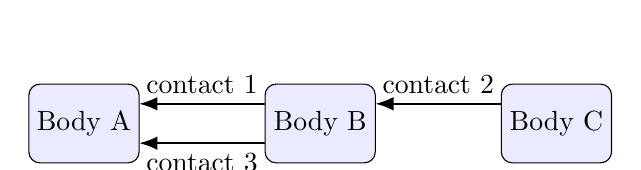
\begin{tikzpicture}[>=Latex]
\foreach \x/\name in {0/A,3/B,6/C}{\draw[fill=blue!8,rounded corners] (\x,0) rectangle +(1.4,1);\node at (\x+.7,.5){Body \name};}
\draw[->,thick] (3,.75)--(1.4,.75) node[midway,above] {contact 1};
\draw[->,thick] (6,.75)--(4.4,.75) node[midway,above] {contact 2};
\draw[->,thick] (3,.25)--(1.4,.25) node[midway,below] {contact 3};
\end{tikzpicture}
\caption{Contacts 1 and 3 have the same body pair but separate lever arms and laws. Contact 2 couples to both through body B.}
\end{figure}

\subsection{An incompatibility that no solver can repair}
A planar body has three upward-normal bottom contacts at horizontal arms $-1,0,1$. Every rigid velocity obeys $u_{n,\rm middle}=(u_{n,\rm left}+u_{n,\rm right})/2$. If incoming normal velocities are all $-1$, local restitution values $(0,1,0)$ request outgoing velocities $(0,1,0)$, violating that identity. No contact impulse can meet all three exact targets. Heterogeneous restitution therefore requires a feasible global endpoint law, explicit target relaxation, or contact compliance/timing. It cannot simply impose arbitrary independent local equalities.

\section{Two distinct ways to close the contact law}
\subsection{A passive endpoint comparator}
For one approaching unrestricted pair contact, use a contact-frame mobility $\bv K$ and a requested velocity target $\bv u_*=-\operatorname{diag}(e_n,e_t,e_s)\bv u^-$. Find
\begin{equation}
\min_{\bv j}\frac12(\bv u^-+\bv K\bv j-\bv u_*)^{\mathsf T}\bv K^{-1}
(\bv u^-+\bv K\bv j-\bv u_*),
\end{equation}
subject to exact normal restitution, compressive impulse, tangential and angular capacity bounds, and $\Delta T\leq0$. Rolling capacity is $|j_s|\leq(\kappa_s/\ell)j_n$ with a physical resistance length $\kappa_s$, independent of the representation length.

A normal-only impulse $j_n=-(1+e_n)u_n^-/K_{nn}$, $j_t=j_s=0$, proves single-pair feasibility for $0\leq e_n\leq1$. Positive-definite $\bv K$ makes the metric objective strictly convex, hence the endpoint minimizer unique. The metric and energy are invariant under consistent changes of $\ell$.

This is a proposed bounded dissipative endpoint approximation. Capacity inequalities do not enforce saturated kinetic Coulomb friction or an authentic intermediate slip path. Choosing a lower dynamic capacity when a requested target exceeds a static capacity is an additional heuristic, explicitly labeled in the implementation. The feasibility and uniqueness arguments do not automatically extend to singular, dependent simultaneous contacts. No novelty is claimed for this comparator.

\subsection{A finite compliant contact reference}
A more physically interpretable route retains contact history. Normal compression is $\delta\geq0$ with $\dot\delta=-u_n$, potential $\Psi_n=k_n\delta^2/2$, and unilateral force
\begin{equation}
F_n=\max(0,k_n\delta+c_n\dot\delta).
\end{equation}
This clipped Kelvin--Voigt example is a deliberately simple reference, not a universal material law. For an active contact,
\begin{equation}
D_n=(F_n-k_n\delta)\dot\delta\geq0.
\end{equation}
On the unclipped branch, $D_n=c_n\dot\delta^2$. If the force is clipped to zero, clipping implies $\dot\delta<0$, so $D_n=-k_n\delta\dot\delta\geq0$.

Tangential motion is represented by an elastic displacement $\bv z_t$ and plastic slip velocity $\bv w_t$:
\begin{align}
\dot{\bv z}_t&=\bv u_t-\bv w_t,\\
\bv F_t&=-k_t\bv z_t-c_t\dot{\bv z}_t,
&\Psi_t&=\tfrac12k_t\|\bv z_t\|^2.
\end{align}
In a sticking elastic branch, $\bv w_t=0$ and $\|\bv F_t\|\leq\mu_t^{\rm st}F_n$. When that trial branch exceeds static capacity, plastic slip is selected with
\begin{equation}
\bv F_t=-\mu_t^{\rm dyn}F_n\frac{\bv w_t}{\|\bv w_t\|},
\qquad 0\leq\mu_t^{\rm dyn}\leq\mu_t^{\rm st}.
\end{equation}
The force opposes actual plastic slip, rather than opposing elastic deformation. Positive $c_t$ makes the local branch computable. A sliding mode and its slip direction are retained until a plastic-slip arrest event; the static threshold is tested only in the elastic branch. This hysteretic event logic avoids repeatedly switching at the static limit. Equal static/dynamic coefficients permit a continuous baseline. In 2D let $F_0=-k_tz_t-c_tu_t$. If $|F_0|$ exceeds the static cap, choose $F_t=\mu_t^{\rm dyn}F_n\operatorname{sign}(F_0)$ and $\dot z_t=(-F_t-k_tz_t)/c_t$. The implied plastic slip has the opposite sign from $F_t$.

Rolling uses an elastic angle $\bv z_s$ and plastic relative angular velocity $\bv w_s$, with
\begin{equation}
\dot{\bv z}_s=\bv\omega_s-\bv w_s,\qquad
\bv\tau_s=-k_s\bv z_s-c_s\dot{\bv z}_s,
\qquad \Psi_s=\tfrac12k_s\|\bv z_s\|^2.
\end{equation}
The static/dynamic moment limits are $\kappa_s^{\rm st}F_n$ and $\kappa_s^{\rm dyn}F_n$. Twisting in 3D can be treated with a separate angular state and limit. This independent-cap reference is phenomenological: a real finite patch may have coupled sliding/twisting/rolling wrench capacity, to be identified from pressure and traction or measurements.

All stored states must be transported objectively with the contact frame. The implemented local test freezes geometry and frame, so it is not a complete rotating-body simulator. With appropriate power-conjugate transport, the elastic-slider balance is
\begin{equation}
\bv F_t\cdot\bv u_t+\dot\Psi_t=-D_t,
\qquad D_t=c_t\|\dot{\bv z}_t\|^2-\bv F_t\cdot\bv w_t\geq0,
\end{equation}
and the angular balance is analogous. Summing body and contact energies gives
\begin{equation}
\boxed{\frac{d}{dt}\left(T+\sum_e\Psi_e\right)
=\mathcal P_{\rm ext}-\sum_e(D_{n,e}+D_{t,e}+D_{s,e}+D_{\rm twist,e}).}
\end{equation}
Elastic rebound now comes from stored energy. Restitution numbers are measured outcomes or calibration targets, rather than simultaneous independent velocity requirements. Remaining contact elastic energy at separation must be explicitly assigned to retained internal modes or unresolved dissipation; deleting history without accounting for that energy is not acceptable.

\section{Heterogeneous surfaces and deformable coarse cells}
\subsection{Material labels are not internal deformation}
A rigid body can have different surface patches with different contact laws. All patches still share the same pose and angular/translational velocity. Splitting a surface into such patches distinguishes coatings or contact geometry but does not introduce strain waves, bending, or internal elastic energy.

To approximate deformation, cells need independent poses and compliant interfaces. In an objective interface frame, let $\bv\xi_{ab}$ contain the retained extension, shear and relative rotation. An elementary passive interface has
\begin{equation}
\Psi_{ab}=\tfrac12\bv\xi_{ab}^{\mathsf T}\bv C_{ab}\bv\xi_{ab},
\qquad \bv C_{ab}\succeq0,\qquad\bv D_{ab}\succeq0,
\end{equation}
with energy-conjugate wrench $-\partial\Psi_{ab}/\partial\bv\xi_{ab}-\bv D_{ab}\dot{\bv\xi}_{ab}$. Interface forces and moments must follow from the objective deformation map, not from unrelated ad hoc forces. For finite rotations, derivatives of that map determine consistent moment transport.

Preserve total mass, center of mass, and inertia, including parallel-axis contributions. Fit static compliance and retained low-frequency modes before fitting impacts. A coarse cell does not automatically reproduce bending, shear, or waves merely because its mass is correct. Substructuring \cite{craig} and bonded/discrete elements \cite{potyondy} are essential comparators.

\subsection{Parameters that can be physically identified}
Effective restitution is usually a property of a contacting pair and process, not a universal number attached independently to each body. A coating may change local response, but geometry, backing stiffness, speed, incidence, incoming spin, and unresolved vibration can also change rebound. Neither reviewer found data establishing universal values for this proposal.

\begin{table}[ht]\centering\small
\begin{tabular}{@{}p{.24\linewidth}p{.65\linewidth}@{}}\toprule
Quantity & Identification experiment or requirement\\\midrule
$m,\inertia$ & Density/geometry integration or inertial measurements; preserve these under subdivision.\\
$k_n,c_n$ & Normal indentation/contact duration and isolated rebound over a stated speed range. Fit the selected unilateral force law, not an unrelated restitution formula.\\
$k_t,c_t,\mu_t^{\rm st},\mu_t^{\rm dyn}$ & Tangential loading, slip onset, and controlled sliding; validate oblique rebound with frozen parameters.\\
$k_s,c_s,\kappa_s^{\rm st},\kappa_s^{\rm dyn}$ & Controlled rolling/angular resistance and patch scale; torque capacity has physical length dimensions.\\
Twisting parameters & Torsional loading of a finite patch, with shared wrench capacity if required.\\
Interface matrices & Static extension/shear/bending and low-frequency modal/decay data for the retained deformation states.\\\bottomrule
\end{tabular}
\caption{Identification requirements. No synthetic value in this draft is claimed to be an authentic material parameter.}
\end{table}

Fit on a training set, freeze the laws, and test held-out locations, speeds, angles and spins. Material-pair tables should respect interchange symmetry and directional/objective conventions. Additional state is justified only when it improves predictions of declared observables. The seven-parameter endpoint proposal cannot in general replace stiffness, contact duration, elastic memory and internal-mode information.

\section{Reproducible calculations completed here}
\subsection{Contact-graph and endpoint diagnostics}
The delivered code assembles a planar graph with full force/couple impulses and separate point edges. It verifies total internal linear and angular momentum about a common origin and the global energy identity. A three-body equal-mass chain with incoming velocities $(1,0,-1)$ produces zero outgoing velocities under the implemented zero-restitution normal projection; the two normal impulses are $(1,1)$. Its normal mobility is
\begin{equation}
\bv K_{nn}=\begin{bmatrix}2&-1\\-1&2\end{bmatrix}.
\end{equation}
A separate analytic elastic solve produces $(-1,0,1)$ with impulses $(2,2)$, demonstrating cross-contact coupling. Redundant contact rows are included in an energy/momentum test; their mobility is singular and is not inverted.

The single-pair passive endpoint comparator satisfies its exact normal target and capacity/energy inequalities. Tests using reference lengths $0.1,1,10$ recover the same physical impulses. This verifies representation invariance for the tested cases, not general frictional material accuracy.

\subsection{A history-dependent local contact example}
A frozen-geometry synthetic local reference uses physical normal/tangential/angular mobility
\begin{equation}
\bv K_{\rm physical}=\begin{bmatrix}2&-0.3&0.2\\-0.3&3&-0.4\\0.2&-0.4&4\end{bmatrix},
\qquad \bv u^-=(-1,0.7,2)^{\mathsf T}.
\end{equation}
Stiffnesses are $(k_n,k_t,k_s)=(10000,4000,30)$, tangential/angular damping $(20,2)$, sliding limits $(0.6,0.4)$ and rolling lengths $(0.03,0.02)$, in consistent example units. Normal damping is numerically calibrated to isolated unit-mobility normal restitution $0.6$, giving $c_n\simeq36.17166$. These are synthetic inputs, not material measurements.

The coupled contact opens at time $0.02227184$ with relative velocity
\[\bv u^+\simeq(0.493860,-0.261169,2.185767)^{\mathsf T}.\]
Its effective normal restitution is about $0.49386$, not the isolated calibration value. Its initial kinetic energy is $0.89909670$, final kinetic energy $0.63437980$, residual contact elastic energy $0.00252639$, and integrated dissipation $0.26219051$. The largest total-energy accounting residual is about $5.1\times10^{-10}$ in these units.

Tangential velocity reverses while relative spin increases; the latter does not imply energy creation because channels are coupled. Ten regression tests pass for graph assembly, global momentum/energy, normal complementarity, endpoint feasibility, reference-length invariance, slider passivity, normal calibration and local compliant energy accounting, retained slip modes, transition refinement, and invalid-mobility rejection. This does not test moving geometry, arbitrary polygon detection, 3D contact patches, or calibrated real impacts.

\subsection{Coarse versus fine layered-rod experiment}
The experiment is a force-driven elastic 1D rod, not a collision. Its length, density and area are one; modulus is one on the left half and four on the right. Uniform cells produce lumped masses and axial springs. Both ends are free, with Gaussian force applied at the left end:
\begin{equation}
F(t)=\frac{1}{\sigma\sqrt{2\pi}}
\exp\left[-\frac{(t-6\sigma)^2}{2\sigma^2}\right].
\end{equation}
The force has effectively unit integrated impulse over the simulated interval $[0,6\sigma+2.5]$. Velocity Verlet uses a step no larger than $0.25h/c_{\max}$ or $\sigma/30$, with $h$ the cell length and $c_{\max}=2$. This is an established lumped spatial discretization, not a new adaptive algorithm.

Reference traces use 2048 elements, with a 1024-element check. Coarse models use 8,16,32,64,128 elements. The main observable is the right-end velocity time history on 5001 common sample times. Relative error is the discrete $L^2$ norm of its difference divided by the reference norm. Reported energy is kinetic plus spring energy.

\begin{table}[ht]\centering
\begin{tabular}{@{}lrrrr@{}}\toprule
Pulse & Cells & Velocity error & Energy difference & Reference check\\\midrule
Broad, $\sigma=0.25$ &16&1.3345\%&0.4043\%&0.0002393\%\\
Broad, $\sigma=0.25$ &32&0.3284\%&0.0998\%&0.0002393\%\\
Sharp, $\sigma=0.015$&16&107.5259\%&23.9313\%&1.3513\%\\
Sharp, $\sigma=0.015$&128&57.3209\%&1.8412\%&1.3513\%\\\bottomrule
\end{tabular}
\caption{Actual synthetic results. ``Reference check'' is the 1024-versus-2048 velocity discrepancy. Energy difference is relative to the fine driven response, not a claim of dissipative loss.}
\end{table}

The broad-pulse result supports accuracy of selected low-bandwidth outputs using coarse cells. The sharp pulse refutes a uniform coarse-accuracy claim. Its reference discrepancy supports identifying order-one coarse failure but does not establish a subpercent converged truth for sharp loading. Integration work--energy residuals are separately recorded in the CSV.

\begin{figure}[ht]\centering
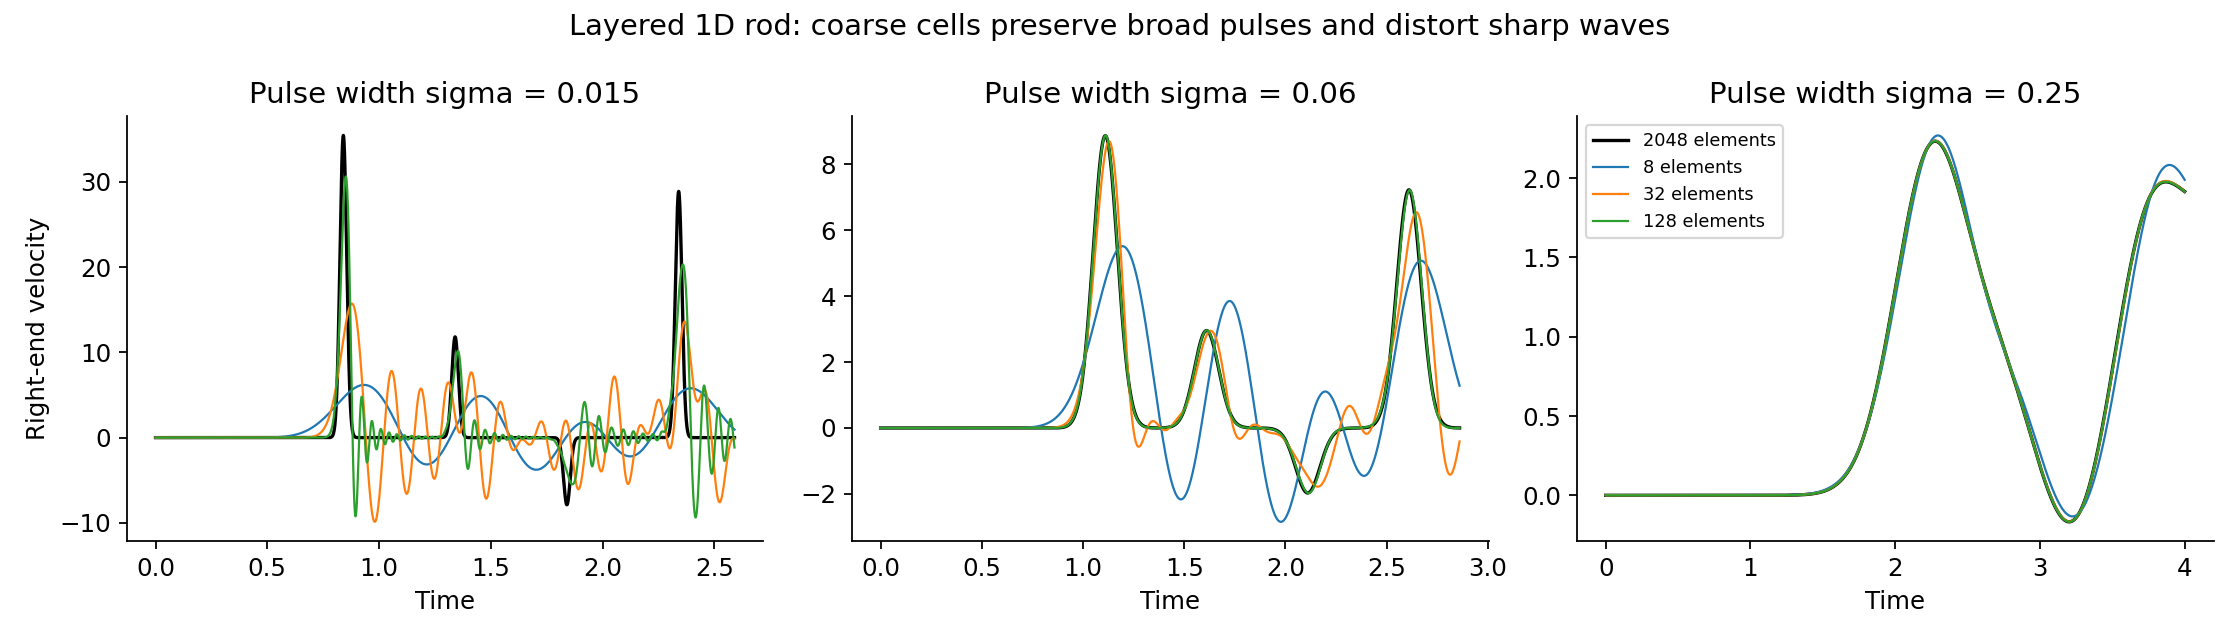
\includegraphics[width=\linewidth]{rod-time-traces.png}
\caption{Right-end velocity under three imposed pulse widths. Coarse cells distort short-wave response. This is not a 2D impact or friction validation.}
\end{figure}
\begin{figure}[ht]\centering
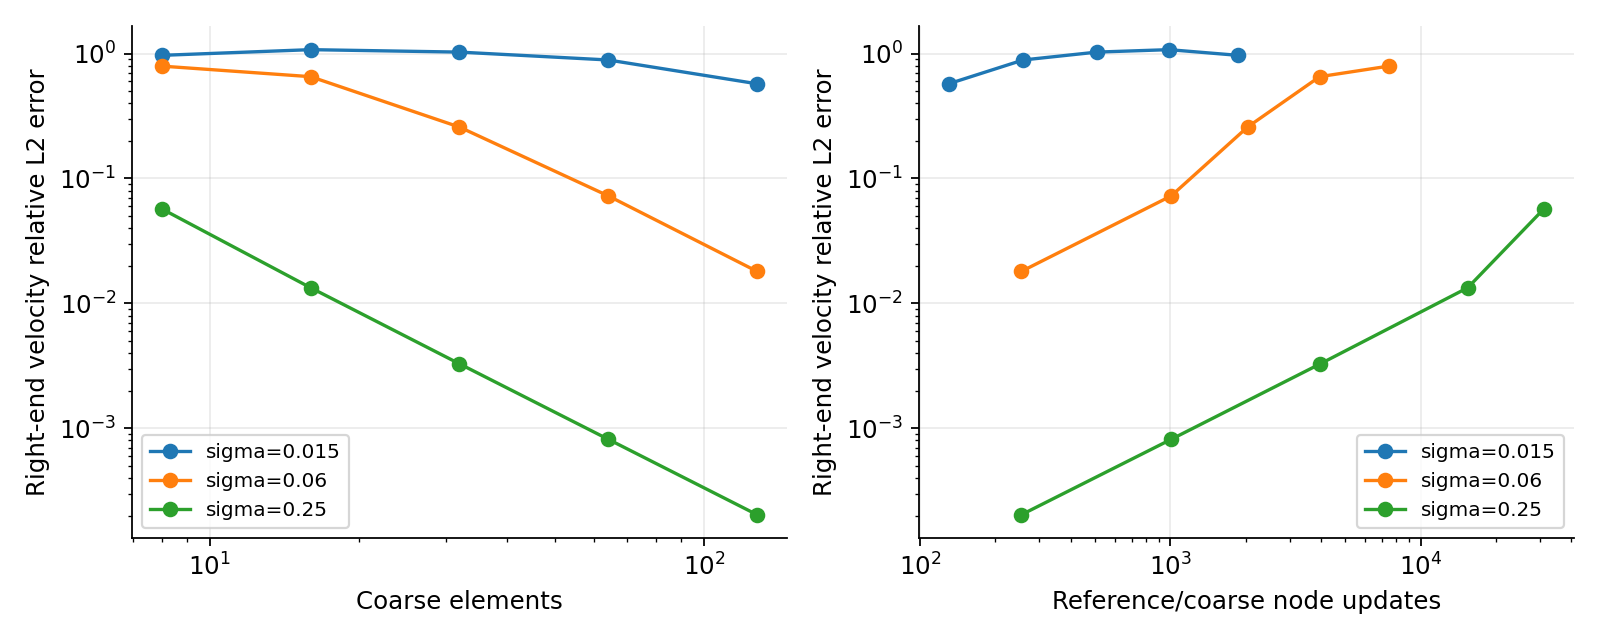
\includegraphics[width=.92\linewidth]{rod-error-cost.png}
\caption{Error versus cell count and arithmetic node-update reduction relative to the explicit 2048-element reference. The reference is deliberately fine; this comparison does not establish superiority over an optimized method at matched error.}
\end{figure}

Single-run wall-clock ratios and node-update counts are available as exploratory diagnostics. They are not robust speedup measurements and omit calibration/adaptation cost. An overresolved explicit reference is not the correct competitor for a claim of practical superiority. The appropriate comparisons include hydroelastic contact, bonded DEM and reduced flexible-body methods.

\section{A testable revised research contribution}
A candidate contribution is an adaptive heterogeneous reduction with an error estimator targeting integrated contact wrench and outgoing center-of-mass velocity/spin. Refine interfaces or patches when material contrast, contact geometry, load bandwidth, or omitted-mode work predicts excessive output error. Merge only while preserving inertial quantities and accounting for stored energy. This proposed adaptive rule is not yet implemented or shown to be novel.

A publication study should predeclare its applicable regime and observables, separate calibration from evaluation, and compare uniform and adaptive variants with close prior art. Tests must cover held-out locations, incident velocities, obliquity, spin, coating boundaries, multiple contacts, prestrain, and internal vibration. Include matched-cost and matched-error curves with preprocessing and calibration included.

Two states with identical exterior rigid contact data but different unresolved internal strain or vibration can have different rebound. A memoryless local restitution table cannot distinguish them. That falsifies a universal memoryless claim, but may motivate retaining a few additional interface/mode states. Those states and their identification cost count toward the reduced model.

A publishable positive result needs a distinct algorithm, theorem, or demonstrated transferable advantage. A clear negative regime boundary or carefully benchmarked limitation could also be scientifically useful, depending on venue and contribution. No superiority result or general novel algorithm has been established here.

\section{Deliverables, status, and remaining limits}
The opposing reviewers' reports and joint verdict accompany this PDF. The code includes planar contact-graph assembly, a frictionless inelastic global reference solver, a single-pair passive endpoint comparator, a local compliant elastic-slider reference, regression tests, and the layered-rod study with raw CSV data.

The contact-history law is fully specified for its local frozen-frame example. The graph gives the general simultaneous assembly. These are not a completed arbitrary-body production simulator: moving contact geometry, finite-patch wrench identification, complete global frictional mode solving, adaptive coarse-cell selection, 3D implementation, and material validation remain open. Numerical convergence and physical authenticity must not be inferred from algebraic energy consistency alone.

The final shared verdict is \textbf{no-go for submitting current novelty claims; conditional go for a narrower research program}. The data supplied here support restricted coarse reduction and reveal meaningful failure cases. A future decision to publish should follow the proposed method and held-out evidence, rather than an advocacy preference.

\begin{thebibliography}{12}
\bibitem{stronge} W. J. Stronge (1990). Rigid body collisions with friction. \emph{Proc. R. Soc. A} 431,169--181. \url{https://doi.org/10.1098/rspa.1990.0125}.
\bibitem{aghili} F. Aghili (online 2019). Energetically consistent model of slipping and sticking frictional impacts in multibody systems. \emph{Multibody System Dynamics}. \url{https://doi.org/10.1007/s11044-019-09703-2}.
\bibitem{maw} N. Maw, J. R. Barber, J. N. Fawcett (1981). The Role of Elastic Tangential Compliance in Oblique Impact. \emph{J. Lubrication Technology} 103,74--80. \url{https://doi.org/10.1115/1.3251617}.
\bibitem{anitescu} M. Anitescu, F. A. Potra (1997). Formulating Dynamic Multi-Rigid-Body Contact Problems with Friction as Solvable Linear Complementarity Problems. \emph{Nonlinear Dynamics} 14,231--247. \url{https://doi.org/10.1023/A:1008292328909}.
\bibitem{elandt} R. Elandt, E. Drumwright, M. Sherman, A. Ruina (2019). A pressure field model for fast, robust approximation of net contact force and moment between nominally rigid objects. \emph{IROS}. \url{https://arxiv.org/abs/1904.11433}; \url{https://doi.org/10.1109/IROS40897.2019.8968548}.
\bibitem{craig} R. R. Craig Jr., M. C. C. Bampton (1968). Coupling of substructures for dynamic analyses. \emph{AIAA Journal}. \url{https://doi.org/10.2514/3.4741}.
\bibitem{potyondy} D. O. Potyondy, P. A. Cundall (2004). A bonded-particle model for rock. \emph{Int. J. Rock Mechanics and Mining Sciences} 41,1329--1364. \url{https://doi.org/10.1016/j.ijrmms.2004.09.011}.
\bibitem{ai} J. Ai, J.-F. Chen, J. M. Rotter, J. Y. Ooi (2011). Assessment of rolling resistance models in discrete element simulations. \emph{Powder Technology} 206,269--282. \url{https://doi.org/10.1016/j.powtec.2010.09.030}.
\bibitem{liu} C. Liu, Z. Zhao, B. Brogliato (2008). Frictionless multiple impacts in multibody systems. I. Theoretical framework. \emph{Proc. R. Soc. A} 464,3193--3211. \url{https://doi.org/10.1098/rspa.2008.0078}. Frictionless scope; not validation of the present angular/friction law.
\end{thebibliography}
\end{document}
